\documentclass[conference]{IEEEtran}
\IEEEoverridecommandlockouts
% The preceding line is only needed to identify funding in the first footnote. If that is unneeded, please comment it out.
\usepackage{cite}
\usepackage{amsmath,amssymb,amsfonts}
\usepackage{graphicx}
\usepackage{textcomp}
\usepackage{xcolor}
\usepackage{subfig}
\usepackage{algorithmic, algorithm}
\usepackage{hyperref}
\usepackage{hyperref} % makes cross-refs (biblio, figures, algos, ...) clickable
\def\BibTeX{{\rm B\kern-.05em{\sc i\kern-.025em b}\kern-.08em
    T\kern-.1667em\lower.7ex\hbox{E}\kern-.125emX}}

\newcommand{\logic}[1]{\color{red}\textbf{Logic/flow:}#1\color{black}}
\newcommand{\writing}[1]{\color{green}\textbf{Writing:}#1\color{black}}
\newcommand{\tristan}[1]{\color{orange}\textbf{From Tristan:}#1\color{black}}
\newcommand{\timothee}[1]{\color{blue}\textbf{From Timothée:}#1\color{black}}

\begin{document}

\title{Repartitioning large multi-dimensional arrays: a sequential algorithm and its implementation in Dask}

\author{\IEEEauthorblockN{Timoth\'ee Gu\'edon, Val\'erie Hayot-Sasson, Tristan Glatard \\
  \IEEEauthorblockA{
    Department of Computer Science and Software Engineering, Concordia University, Montreal, Canada
  }}
}

\maketitle

\begin{abstract}
Todo.
\end{abstract}

\begin{IEEEkeywords}
multidimensional, array, split, merge, resplit, IO, processing, Dask, Python
\end{IEEEkeywords}

%----------------------------------------
\section{Introduction}
%----------------------------------------
% big data challenges
With the improvement of acquisition methods and the growth in the amount of data
available in several scientific domains such as health
sciences~\cite{bigdata_health}~\cite{Amunts1472}, geology~\cite{big_data_geology}
and astrophysics~\cite{biguniverse}, new big data challenges have emerged related
to the processing of large amounts of data and ultra-high resolution
images. Big Brain, a human brain model providing microscopic data (20 micrometers) for
modeling and simulation~\cite{Amunts1472} is an example of ultra high resolution
images in the neuroscience field.

\subsection{Data storage on disk}
% use of chunking
Scientific data is often represented as multidimensional arrays stored in
chunks to facilitate processing and storage. Among other advantages, chunking
allows for efficient queries, flexibility in adding new
data~\cite{optimal_chuking}, parallel processing, and out-of-core
computations through block algorithms~\cite{matthew_rocklin-proc-scipy-2015}.

% explain storage order
Previous work focused on optimizing the data storage by looking for an optimal
chunk shape that would reduce the expected number of chunks to be retrieved by
any query~\cite{optimal_chuking} or by optimizing the ordering of the chunks
using space filling curves for example~\cite{optimal_chuking, openconnectomecluster}.
Instead, our approach is to leave the choice of the
data storage to the application as much as possible, as in~\cite{seqalgorithms}.
We therefore assume that the chunk shape and the data ordering in files are
arbitrary but known.

For the sake of clarity and without loss of generality,
 we assume in this study that files are written in row-major order (a.k.a
``C" order), where the fastest moving dimension in the file is the last
dimension in the array, and the slowest moving dimension in the file is the first
dimension in the array. For example a 3D array with dimensions $i$, $j$ and $k$
would be written on disk by writing the complete columns in the k dimension first
(see Figure~\ref{fig:seeks_and_rowmajor} (a)).
Our experiments use the HDF5~\cite{hdf5} file format as it is commonly used in the
scientific community and it is written in \texttt{C-order} by default.

\begin{figure*}[h]
  \centering
  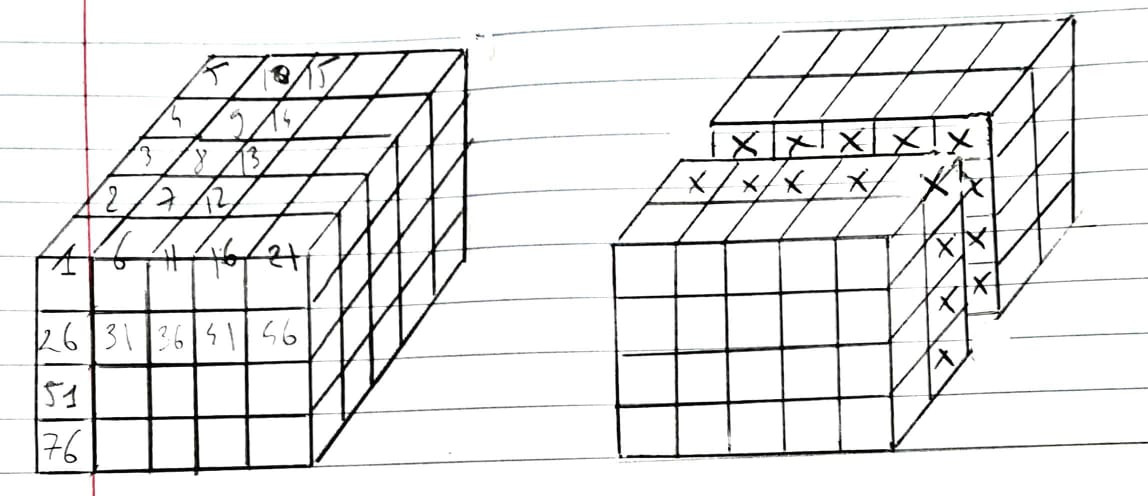
\includegraphics[scale=0.35]{./figures/new/seeks_and_rowmajor.jpeg}
  \caption{Illustration of the r\texttt{C-order} in files. The left subfigure
  shows how the data is written on disk, with each cube representing a voxel. The
  right subfigure shows how reading or writing only one part of a cuboid written
  in the \texttt{C-order} can produce seeks. Each cross represents a seek.}
  \label{fig:seeks_and_rowmajor}
\end{figure*}

\subsection{Multidimensional array chunking}

% need for tools to repartition
Using chunked multidimensional arrays requires tools to efficiently split,
merge, and ``resplit" or ``repartition" data files. Previous work in~\cite{seqalgorithms}
showed that naive algorithms to split an array into several chunks or merge
array chunks into one output file do not perform well due to millions of seeks
occurring on disk. The present study is focused on sequential algorithms for
repartitioning multidimensional arrays, letting the parallel and distributed
cases as future work, although they are relevant, too. To the best of our
knowledge, the repartition problem has not been extensively studied.

% why subarray extraction incurs seeks
Retrieving sub-arrays from an array stored on disk incurs seeks in two
situations: (1) when an array block is opened for reading or writing, and (2)
when the reading or writing process moves within the block to access a
contiguous piece of data. For a 3D cuboid of shape $C = (C_i, C_j, C_k)$ stored
in row-major order, each column of data in the k dimension is contiguously
stored. There are therefore $C_j \times C_i$ data columns that all require a
seek (see Figure~\ref{fig:seeks_and_rowmajor} (b)).
Although the seek time depends on various parameters such as the distance
in bytes between two data columns, we assume that all seeks incur the same time
overhead for the sake of simplicity. Therefore our problem will be to minimize
the number of seeks required to access data.

Not only extracting a subarray from a chunk incurs seeks on disk, but also
accessing any piece of data from a chunk results in loading the whole chunk in
memory. Chunking must therefore be used with care as it can be detrimental for
performance. The Python library \texttt{h5py} for manipulating HDF5 files
recommends a chunk size ``between 10 KiB and 1 MiB" and more for larger
datasets~\cite{collette_2014}. \texttt{dask}, a popular Python package, part of
the SciPy ecosystem, enabling parallel and out-of-core
computations~\cite{matthew_rocklin-proc-scipy-2015} also mentions the issues
relative to chunking and suggests a chunk size greater than 100 MB, although
remainding that the chunk shape selection is highly dependent on the
application~\cite{rocklin_bourbeau_2019}.

\subsection{Contributions}
This paper makes the following contributions:
\begin{itemize}
  \item The definition of the re-partition problem for multidimensional arrays
  \item The proposition of a sequential algorithm to efficiently
  re-partition multidimensional arrays
  \item An open implementation of this algorithm on Github
\end{itemize}

\section{Problem definition}
\subsection{The re-partition problem}
We focus on 3D arrays for simplicity. Consider a 3D array of shape $R =
(R_i, R_j, R_k)$, partitioned as input chunks of uniform shape $I = (I_i,
I_j, I_k)$ stored on disk. Our goal is to re-partition the input blocks into
output blocks of uniform but different shape $O = (O_i, O_j, O_k)$.
A re-partitioning algorithm reads the input blocks from disk, and writes the
output blocks to disk.

We present hereafter a general algorithm for the re-partition task.

A re-partioning algorithm (Algorithm~\ref{algo:generalrepartition}) takes a
list of input blocks \texttt{inBlocks} of shape $I$, a list of output block
definitions \texttt{outBlocks} of shape $O$ and the amount of memory \texttt{m}
available for the algorithm.
Subject to $m$, the algorithm first defines a list of buffers, the
\texttt{readBuffers}, to read from the input blocks (line 9).
These buffers have the same shape $B$.
Then, the algorithm computes another list of buffers, the \texttt{writeBuffers},
in which each buffer is a piece of data to be written at a time into an
output file (line 10).
In other words, the write buffers describe how each output file will be written.
All readBuffers have the same shape $B$. On the contrary, the writeBuffers can
have different shapes.
Finally, the main loop of the algorithm (line 12) loads one readBuffer at a
time (line 13), inserts it into a cache (line 14), and writes each writeBuffer
as soon as its data is available in cache (lines 15 to 18).

For simplicity, we require that all buffers in \texttt{readBuffers} have
the same shape $B$. We define the cost function $\mathrm{seeks}$ as returning
the number of seeks incurred by the repartitioning algorithm.
The re-partitioning problem is therefore to find the best read and write buffers
lists in order to minimize $\mathrm{seeks}$ subject to $m$.
Solutions of this problem materialize as implementations of function
\texttt{getReadBuffers} and \texttt{getWriteBuffers} in
Algorithm~\ref{algo:generalrepartition}.

A lower bound on the number of seeks for the repartitioning problem is
$n_i + n_o$, with $n_i$ the number of input files and $n_o$ the number of output
files. Indeed, input and output files all have to be accessed at least once,
which requires a seek.

\begin{algorithm}
  \caption{General re-partitioning algorithm}
  \label{algo:generalrepartition}
  \begin{algorithmic}[1]
    \STATE \textbf{Inputs}
    \STATE inBlocks: input chunks stored in one dedicated file (or in one dataset of a HDF5 file).
    \STATE outBlocks: output chunks to be written, created as one empty file (/dataset of a HDF5 output file).
    \STATE $m$: memory available for one readBuffer or writeBuffer
    \STATE $I$: shape of one input chunk
    \STATE $O$: shape of one output chunk
    \STATE
    \STATE \textbf{Algorithm}
    \STATE B, readBuffers $\leftarrow$ getReadBuffers($I$,$O$,$m$)
    \STATE writeBuffers $\leftarrow$ getWriteBuffers($O$, $B$)
    \STATE initialize(cache)
    \FOR{readBuffer in readBuffers}
      \STATE bufferData $\leftarrow$ read(readBuffer, inBlocks)
      \STATE cache.insert(bufferData)
      \FOR{writeBuffer in writeBuffers}
        \IF{cache.isComplete(writeBuffer)}
          \STATE data = cache.pop(writeBuffer)
          \STATE write(writeBuffer, outBlocks)
        \ENDIF
      \ENDFOR
    \ENDFOR

  \end{algorithmic}
\end{algorithm}

\subsection{The multiple and clustered strategies}
Special cases of the re-partitioning problem occur when $I=R$ (``split'' problem)
or when $O=R$ (``merge'' problem). Two strategies were introduced
in~\cite{seqalgorithms} to address these problems: the ``multiple" and the
``clustered" strategies. In these strategies, every loaded buffer is directly written to the
destination output files.
The only difference between the multiple and the clustered strategies lies in
the selection of $B$.

In the split problem studied in~\cite{seqalgorithms} ($I=R$), a \texttt{naive}
strategy defines the read buffers as having the same shape than the output blocks
($B$=$O$). The read buffers are iteratively loaded from $R$ and entirely written
to the appropriate output block (represented by a writeBuffer of shape $O$, too).
The \texttt{clustered} strategy, however, loads as
many contiguous data blocks of shape $O$ as possible to fit in $m$.
$B$ is therefore a multiple of $O$.
Depending on the amount of main memory available, the data blocks may be loaded
individually, by entire block columns, or by entire block slabs.
Although this strategy allows to write each output block in one seek
(for opening the output file), the clustered strategy is limited by the fact
that it does not optimize the reading step.
In the case of the re-partition task, one can expect the clustered strategy to
perform poorly as
(1) it reads an output block no matter if it is split in a lot of different input blocks
and (2) even if it is stored in one input block the algorithm will do a lot of seeks in
case of a shape mismatch.
These limits are exacerbated in the re-partition task as there are many input and
output files.

The \texttt{multiple} strategy used for the split problem in~\cite{seqalgorithms}
aims at not doing any seek while reading \textit{and} writing;
Both the input and the output blocks are read/written contiguously. In
terms of Algorithm~\ref{algo:generalrepartition}, this means defining read buffers as
contiguous parts of the input array and write buffers as contiguous parts of
the output arrays. It is equivalent to extending the buffer in the inverse of
the storage order: $k \rightarrow j \rightarrow i$ in the case
of the \texttt{C-order}. The tradeoff lies in switching between files
at each buffer loading. In this case too, using this strategy for the re-partition task would
result in even more switches between input and output files which makes the limit
even more important.

To the best of our knowledge, no algorithm has been proposed for the
repartitioning task.

\subsection{Baseline solution}

Our baseline algorithm for the repartitioning problem loads one input block
at a time, that is, $B$=$I$ in Algorithm~\ref{algo:generalrepartition},
and directly writes it to the appropriate output blocks.
The write buffers are therefore defined by the intersections between the input
and output blocks.
For the baseline algorithm, we assume that one input block fits in memory ($m \geq I_iI_jI_k$).
As in Algorithm~\ref{algo:generalrepartition}, each buffer is only loaded once.

The number of seeks $s$ induced by this baseline algorithm is the
sum of the number of seeks done for each buffer, that is, the sum of:
\begin{itemize}
  \item the number of input blocks (1 seek per read buffer)
  \item the number of output blocks openings
  \item the number of seeks done by writing into the output blocks
\end{itemize}

We say that there is a \emph{shape mismatch} in a given dimension $x$ if the
border of an output block does not match the border of an input block, and
vice versa.
Considering a shape mismatch in the dimension $k$, we can represent it as a cut
into the whole image of shape $R$ which will incur $R_iR_j$ seeks. Using the
same reasoning, a cut in dimension $j$ will incur $R_i$ seeks and a cut in
dimension $i$ will only incur 1 seek.
It is also worth noticing that if there is a cut in dimension k and j, the seeks
produced by the cut in $j$ will be included in the seeks produced in dimension $k$.
The same reasoning applies to $i$ and $j$.
From this observation we can compute the number of seeks $s$ produced as:

\begin{equation} \label{eq:1}
s = R_i R_j c_k + R_i c_j m_k + c_i m_j m_k + N
\end{equation}

With $c_x$ the number of cuts (shape mismatches) in dimension $x$, $m_x$ the
number of shape matches. The first component corresponds to the seeks produced
by the shape mismatches in $k$, the second component to those in $j$ and the last
component by the mismatches in $i$. Finally, $N$ designates the number of input files.

It seems from Equation~\ref{eq:1} that unless the dimensions of the input and
output files match, a considerable amount of seeks will occur, the number of
seeks being factors of $R_j$ and/or $R_i$. Also, a shape mismatch in the
$k$ dimension should be more costly than a shape mismatch in the $j$ dimension,
which is itself more costly than a mismatch in dimension $i$ (assuming that the
files are stored in C-order).

We implemented Equation~\ref{eq:1} and ran it on a cubic array to confirm these
theories. One shape mismatch is added at a time in order to see the impact on
the number of seeks. The setting and results of this simulation are summarized
in table~\ref{tab:simseekmodel}.

\begin{table}[ht]
  \centering
  \caption{Results of the simulation using the baseline algorithm's seek model}

   \begin{tabular}[t]{c c c c c }
   \hline
   Mismatch & R & B=I & O & nb seeks \\
     \hline\hline
     k & (3500,3500,3500) & (500,500,875) & (500,500,500) & 73,500,000 \\
     \hline
     j & (3500,3500,3500) & (500,875,500) & (500,500,500) & 147,000 \\
     \hline
     i & (3500,3500,3500) & (875,500,500) & (500,500,500) & 294 \\
     \hline
     i,j & (3500,3500,3500) & (875,875,500) & (500,500,500) & 147,168 \\
     \hline
     i,j,k & (3500,3500,3500) & (875,875,875) & (500,500,500) & 73,584,096 \\
     \hline
   \end{tabular}

   \label{tab:simseekmodel}

\end{table}

%----------------------------------------
\section{The ``keep" algorithm}
%----------------------------------------

\subsection{The keep strategy}

As mentioned previously, like the split and merge strategies the baseline
algorithm for the repartition problem empties the cache at each iteration. In a
split/merge/repartition problem a lot of seeks occur in case of a shape mismatch,
for example, when a data column loaded in memory is split between two output
files or more. We propose to leverage the cache using a \texttt{keep strategy}
to keep some data in the cache while it cannot be written contiguously in output
files~\ref{fig:keepvsbaseline}.

\begin{figure}[h]
\centering
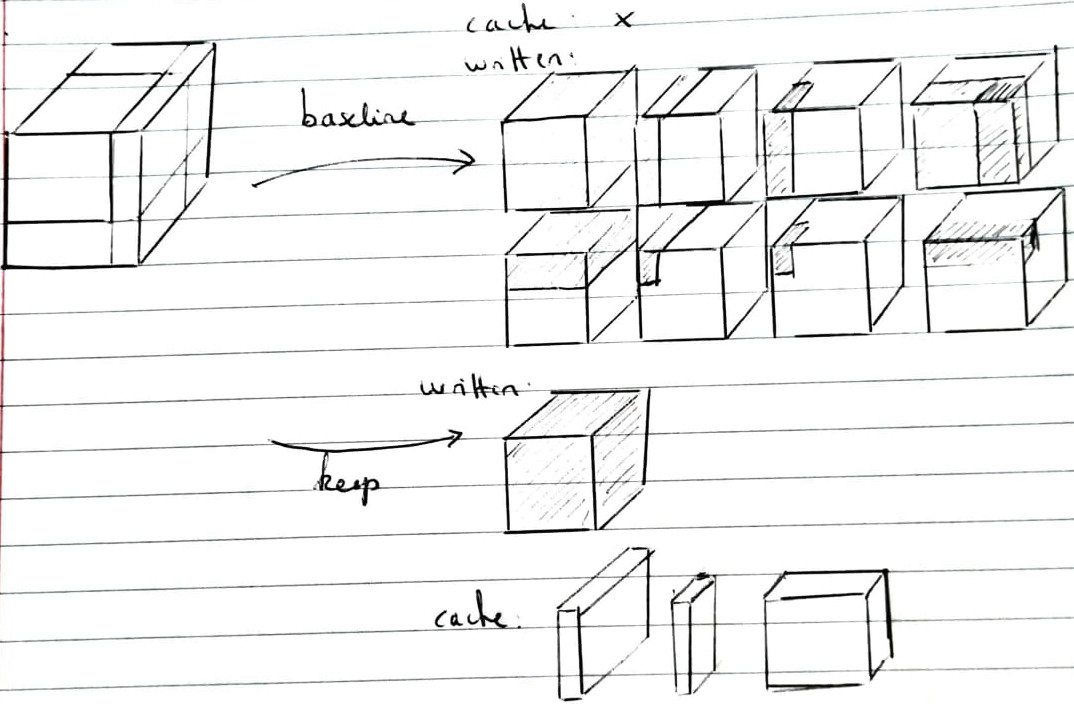
\includegraphics[scale=0.25]{./figures/new/naive_vs_keep.jpeg}
\caption{desc.}
\label{fig:keepvsbaseline}
\end{figure}

In the cache (Algorithm~\ref{algo:generalrepartition}), the data that is not
contiguous in its output file of destination is called \texttt{extra data}.
The \texttt{keep strategy} first consists in finding a buffer shape covering at least
one output file completely, i.e. $B_x>O_x$ for all dimensions $x$.
Such a buffer shape would allow to always have extra data in case of a shape
mismatch, hence making the cache management possible to reduce the number of seeks.
We call this ideal buffer shape an \texttt{input aggregate}, which shape is
written $\Lambda$. Using such an optimal buffer shape and being able to keep all
the extra data into memory during the whole repartition algorithm would incur
the minimum number of seeks possible: $n_i + n_o$. Indeed, it is equivalent to
writing an output file only when all its data is in cache.
If $m$ is too small, then the keep strategy tries to find a buffer
shape as closed as possible from $\Lambda$.

\subsection{The keep algorithm}

The implementation of the keep strategy is equivalent to implementing
\texttt{getBufferPositions} in Algorithm~\ref{algo:generalrepartition} to find a
buffer shape closed to the optimal buffer shape $\Lambda$. Such an implementation is
presented in Algorithm~\ref{algo:getbuffersposition}. The implementation
consists in extending the buffer shape, initialized as $B=(1,1,\Lambda_k)$ (line 13), in
one dimension at a time. Because of its initialization, $B_k=\Lambda_k$, therefore
the buffer needs to be extended in the $i$ and $j$ dimensions only (in 3D).
From line 14 to 22 the buffer is extended in the $j$
dimension, and from line 23 to 31 the buffer is extended in the $i$ dimension.
Finally, the coordinates list of each buffer is computed from the buffer shape
that has been found. At each step of the buffer extension \texttt{volumesToKeep}
is computed to define which part of extra data will have to be kept in memory.
The next subsections explain each part of Algorithm~\ref{algo:getbuffersposition}
in details.

\begin{algorithm}
  \caption{The keep algorithm - Pseudocode of the \texttt{getBufferPositions} function for the keep strategy}
  \label{algo:getbuffersposition}
  \begin{algorithmic}[1]
  \STATE \textbf{Inputs}
  \STATE $\Omega_{max}$: tuple of the maximum overlap length
  of any buffer in all dimensions,
  \STATE $\Lambda$: input aggregate shape,
  \STATE $m$: amount of available memory for the buffer
  \STATE
  \STATE \textbf{Outputs}
  \STATE \texttt{buffersList} the coordinates of all buffers to be loaded,
  \STATE \texttt{policy} the policy to be used for the cache management by \texttt{getDataToWrite}
  \STATE
  \STATE \textbf{Algorithm}

  \STATE $\Omega \leftarrow \Omega_{max}$
  \STATE $\Theta = (\Lambda_i - \Omega_i, \Lambda_j - \Omega_j, \Lambda_k - \Omega_k)$
  \STATE $B \leftarrow (1,1,\Lambda_k)$

  \STATE $\phi = \lfloor \frac{m}{\Omega_k + \Lambda_k} \rfloor$ // keeping $F_1$
  \STATE $B_j = \begin{cases}
    \Theta_j & \textrm{if }\phi \geq \Theta_j \\
    1 & \textrm{if }\phi = 0 \\
    \phi & \textrm{else}
  \end{cases}$

  \IF{$B_j \neq \Theta_j$}
    \STATE volumesToKeep = [1] // if cannot store $F_1$ entirely, stop the algorithm
  \ELSE
    \STATE $\phi = \lfloor \frac{m-\Theta_j(\Omega_k\Lambda_k)}{\Lambda_k(n+1)} \rfloor$  // keeping $F_1$, $F_2$ and $F_3$
    \STATE $B_j = \begin{cases}
      \Lambda_j & \textrm{if }\phi \geq \Lambda_j \\
      B_j & \textrm{if }(B_j+\phi) = 0 \\
      B_j + \phi & \textrm{else}
    \end{cases}$

    \IF{$B_j \neq \Lambda_j$}
      \STATE volumesToKeep = [1,2,3]
    \ELSE
      \STATE $\phi = \lfloor \frac{m}{\Omega_k\Theta_j + n\Omega_j\Lambda_k + \Lambda_j\Lambda_k} \rfloor$ // extending $F_1$, $F_2$ and $F_3$ in dimension $i$
      \STATE $B_i = \begin{cases}
        \Theta_i & \textrm{if }\phi \geq \Theta_i \\
        1 & \textrm{if }\phi = 0 \\
        \phi & \textrm{else}
      \end{cases}$

      \IF{$B_i \neq \Theta_i$}
        \STATE volumesToKeep = [1,2,3]
      \ELSE
        \STATE $\phi = \lfloor \frac{m-\Theta_i(\Omega_k\Theta_j + n\Omega_j\Lambda_k + \Lambda_j\Lambda_k)}{(N+1)\Lambda_j\Lambda_k} \rfloor$ // keeping $F_1$ to $F_7$
        \STATE $B_i = \begin{cases}
          \Lambda_i & \textrm{if }(B_i+\phi) \geq \Lambda_i \\
          B_i & \textrm{if }\phi = 0 \\
          B_i+\phi & \textrm{else}
        \end{cases}$

        \STATE volumesToKeep = [1,2,3,4,5,6,7]
      \ENDIF
    \ENDIF
  \ENDIF

  \STATE policy $\leftarrow$ getPolicy(volumesToKeep)
  \STATE buffersList $\leftarrow$ getBuffersCoordinates($B$)
  \RETURN buffersList, policy
  \end{algorithmic}
\end{algorithm}

\subsection{Input aggregates}
Our goal is to find the optimal buffer shape such that $B_x>O_x$ in any dimension $x$.
If $I_x > O_x$, then $B_x$ can be set to $I_x$. If $I_x < O_x$ however, $B_x$
must be a multiple of $I_x$ in order to keep reading each input file in one seek.
We define an \texttt{input aggregate} as being the minimum aggregate of input files that
covers one output file completely. In particular, it is the input aggregate that
covers the first output file (indexed $(0,0,0)$) in the original image being
repartitioned. The best buffer shape for the keep strategy is therefore the shape of
an input aggregate.

\subsection{Stretching the buffer in the inverse storage order}
To get a buffer shape close to $\Lambda$ we define an algorithm
\texttt{getBufferShape} in \texttt{getBufferPositions} that stretches the
buffer shape step by step. At each step, the algorithm estimates how much the
buffer can be stretched in one direction while keeping the remainders into
memory. The problem of what dimension to increase first still stands. A
strategic order seems to be to stretch the buffer in the direction which saves
the maximum number of seeks first. Given the analysis of the baseline algorithm,
such an order is the inverse of the storage order i.e.
$k \rightarrow j \rightarrow i$ for the \texttt{C-order}.

\subsection{Impact of the buffer order on performance}
Using the keep strategy, one may order the buffer loadings to reduce the maximum
quantity of extra data stored in memory, hence, reducing the amount of seeks.
For example, if an overlap occurs only in the $k$ axis, loading the next buffers
in this direction will enable recycling the extra data kept in memory, resulting
in a smallest memory consumption over time. The memory saved thanks to a smart
ordering could enable the storage of more overlaps in memory using the
``keep strategy", further reducing the overall number of seeks.

As explained in the discussion, the buffer ordering problem is complex and does
not seem easily solvable.
This study uses a naive order which is the storage order. Note that using such
an order allows recycling extra data in the $k$ dimension first, it is therefore
most efficient when the biggest overlap between input and output files is in the
$k$ dimension.

Thanksfully, the impact of the buffer ordering on performance can be
mitigated. Indeed, the impact of the buffer ordering depends on the size of the
mismatches. One can reduce the amount of extra data by using smallest chunks: Even
if the overlap between the input and output files is big with respect to their
size, the area/volume of the overlap will be kept small.

\subsection{The buffer extension}

The buffer extension aims at extending the buffer shape from
(1,1,$\Lambda_k$) to the input aggregate shape $\Lambda$. Note that we assume
that $m$ is large enough to store a buffer of shape (1,1,$\Lambda_k$). It means
that we can read one complete data column from an input file and keep the
remainder in memory for the next buffer. If it was not the case the keep
algorithm would not give a significant improvement in the number of seeks
produced by the repartition task, compared to the baseline algorithm.

In this analysis, we express the quantity of memory used by an array as the
number of voxels it contains. It is equivalent to saying that the number of
bytes per voxel is 1. With $\alpha$ the number of bytes per voxel in the storage
device, $m$ is defined as $m/\alpha$ in the following computations.

The following subsections cover how we estimate the amount of memory required
by the keep strategy to know how much the buffer can be stretched in a given
direction while keeping the extra data in memory. The amount of memory required
is the maximum memory consumption reached during the execution of the keep algorithm.
To estimate this amount, we first need to define what a remainder volume is.

\subsection{Remainder volumes}

A buffer of shape $\Lambda$ can be divided in
8 parts or ``volumes" (Figure~\ref{fig:nomenclature_overlaps}).
7 out of these 8 volumes are called \texttt{remainder volumes} because
they represent the overlap between the input files and the output files on
the buffer borders. These 7 remainder volumes enclose an 8th part that is composed of
input files that are either complete or which complementary part have already
been loaded by a previous buffer. This means that any complementary part is either
in memory (it has been kept in cache according to the keep strategy) or it has
been written down previously. Therefore, this 8th volume cannot be kept by the
keep strategy and is not considered a remainder. For each buffer, each of volume
is indexed following the buffer order $F_0$ to $F_7$, with $F_0$ being the
non-remainder volume. If the buffer is smallest than the input aggregate or if
there is no shape mismatch in a given dimension, it may be that a volume size
is set to 0.

\begin{figure*}[h]
\centering
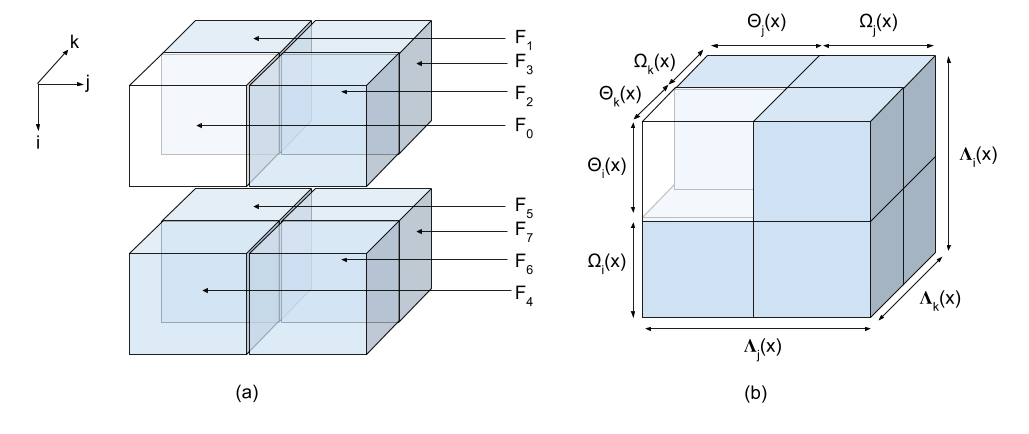
\includegraphics[scale=0.4]{./figures/new/nomenclature_overlaps.png}
\caption{Division of a buffer into 8 parts indexed according to the storage
order, 7 of which are remainder volumes.}
\label{fig:nomenclature_overlaps}
\end{figure*}

\subsection{Maximum memory consumption}

Having partitioned the buffers into volumes, the maximum memory consumption is
computed from two pieces of information: The maximum number of each volume we
must keep during the process and the maximum size of each volume.

In the buffer extension algorithm, the buffer is stretched in one dimension at
a time (Figure~\ref{fig:bufferextensionalgo}).
When stretching the buffer, we compute the maximum length of the buffer possible
in the dimension considered, while ensuring that the remainder volumes can be
kept into memory according to the \texttt{keep} algorithm. For example, if
we consider stretching the buffer in the $j$ dimension, we want to know how big
$B_j$ can be such that the remainders are kept in memory by the \texttt{keep}
algorithm for later use, given the maximum amount of memory available, $m$.

\begin{figure*}[h]
\centering
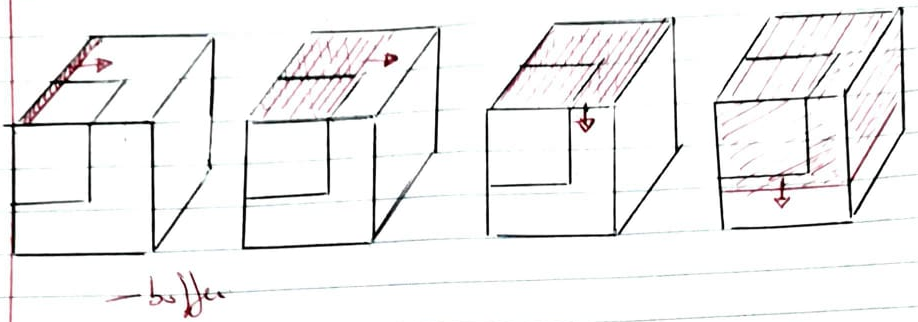
\includegraphics[scale=0.4]{./figures/new/bufferextensionalgo.png}
\caption{desc.}
\label{fig:bufferextensionalgo}
\end{figure*}

$\Sigma$, the maximum amount of data reached during the execution of the keep
algorithm is defined in terms of the number of volumes to keep in cache. From the
previous sections we assume that the buffer order is the storage order.
In this order, the $F_1$ volume stored from a given buffer loading is recycled
in the next one (Figure~\ref{fig:calculmemoire}). Therefore there can be only
one $F_1$ volume in cache at a
given time. $F_2$ and $F_3$ are kept in memory until the next
buffer in the $j$ dimension recyles them. Therefore they can be present in cache
$n$ times at a maximum, with $n$ the number of buffers in a buffer column (the
number of buffers in dimension $k$). Volumes 4 to 7 can only be recycled by the
next buffer in the $i$ dimension. Therefore, the algorithm must read an entire
buffer slice before being able to remove them from the cache. They are kept a
maximum of $N$ times, with $N$ the number of buffers in a slice of the
reconstructed image (Figure~\ref{fig:calculmemoire}).
Last but not least, a buffer must be loaded at each step of
the keep algorithm. This gives us the following formula for $\Sigma$:

\begin{equation} \label{eq:2}
\Sigma = F_1 + n(F_2 + F_3) + N(F_4 + F_5 + F_6 + F_7) + B_iB_jB_k
\end{equation}

\begin{figure}[h]
\centering
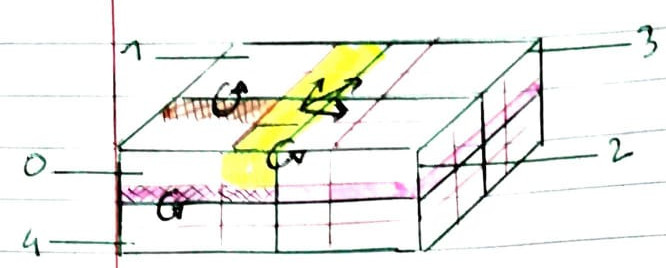
\includegraphics[scale=0.3]{./figures/new/bufferextensionalgoformula.jpeg}
\caption{desc.}
\label{fig:calculmemoire}
\end{figure}

Now that we have an expression for $\Sigma$, we must find its maximum value by
computing the volumes' sizes and their maximum.

\subsection{The getBufferPositions function}

In order to compute $\Sigma$, the volumes' sizes need to be computed using the
following nomenclature (Figure~\ref{fig:nomenclature_overlaps}):
Given a buffer shape $B$ and the output file shape $O$, we define $C_d(x)$ as
the overlap length between the buffer and an overlaping output file in direction
$d$ for the $x^{th}$ buffer. Let us define $\Omega$ and $\Theta$, that are used
to define upper bounds in the volumes sizes formulas. $\Omega_d(x)$ is the
equivalent of $C_d(x)$ if the buffer was of shape $\Lambda$, and $\Theta_k(x)$
is the difference between $B_d$ and $\Omega_b$, with $B=\Lambda$.
These metrics are computed as follows:
$$C_d(x) = (x+1)B_d mod(O_d)$$
$$\Omega_d(x) = (x+1)\Lambda_d mod(O_d)$$
$$\Theta_d(x) = \Lambda_d - \Omega_d(x)$$

The volumes sizes are computed in Appendix~\ref{bufferExtensionAlgorithm}.
Finally, to find the maximum size
of each volume one must know the maximum overlap length between the buffer and
the output files on its border. One can either compute all possibilities and
take the maximum in each dimension if it is not too costly or use the following
upper bound: By definition of an input aggregate, the overlap between any buffer
and its bordering output files it at maximum $O_x$ in dimension $x$. Once the
maximum volumes' sizes are found they can be replaced in $\Sigma$ to find the
maximum memory consumption of the keep algorithm.

Given equation~\ref{eq:2} and the maximum size of the volumes, we can now
stretch the buffer shape one dimension at a time using simple equations to ensure
that the maximum amount of memory consumed during the process will stay below the
amount of memory available. Such computations are given in
Appendix~\ref{bufferExtensionAlgorithm}.
Algorithm~\ref{algo:bufferextensionalgorihm} summarizes the computations into a
pseudocode for the buffer extension algorithm which returns two pieces of
information: the best buffer shape affordable given $m$ and the indices of the
remainder volumes that can be kept in cache. The maximum value that the buffer
can take at any step of the algorithm is represented by $\phi$ (lines 6, 11,
16, 21).

Now that the best buffer shape can be computed, we can express the
\texttt{getBufferPositions} function (Algorithm~\ref{algo:generalrepartition}) in
Algorithm~\ref{algo:getbuffersposition}.

%----------------------------------------
\section{Implementation}
%----------------------------------------

\subsection{Clustered strategy}

As explained in the introduction, \texttt{dask} represents computations by a task graph.
Implementing the clustered strategy consisted in modifying that graph. To that
aim, we implemented an optimization function to create ``buffer" tasks in the
graph (Figure~\ref{fig:bufferization}).

\begin{figure*}
  \centering

  \subfloat[\texttt{dask} graph for splitting a multidimensional array.]{{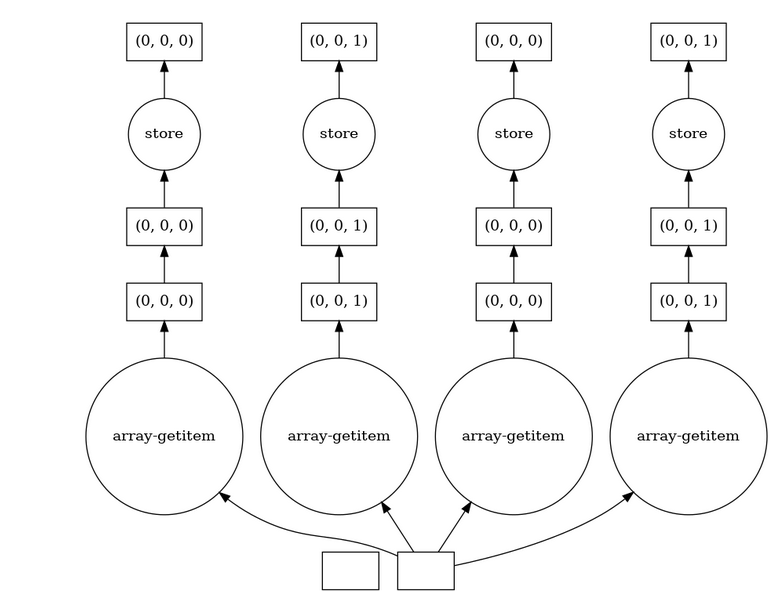
\includegraphics[width=8cm]{./figures/new/before_store.png} }}
  \qquad
  \subfloat[Same \texttt{dask} graph after creating a buffer task (\texttt{merged part}).]{{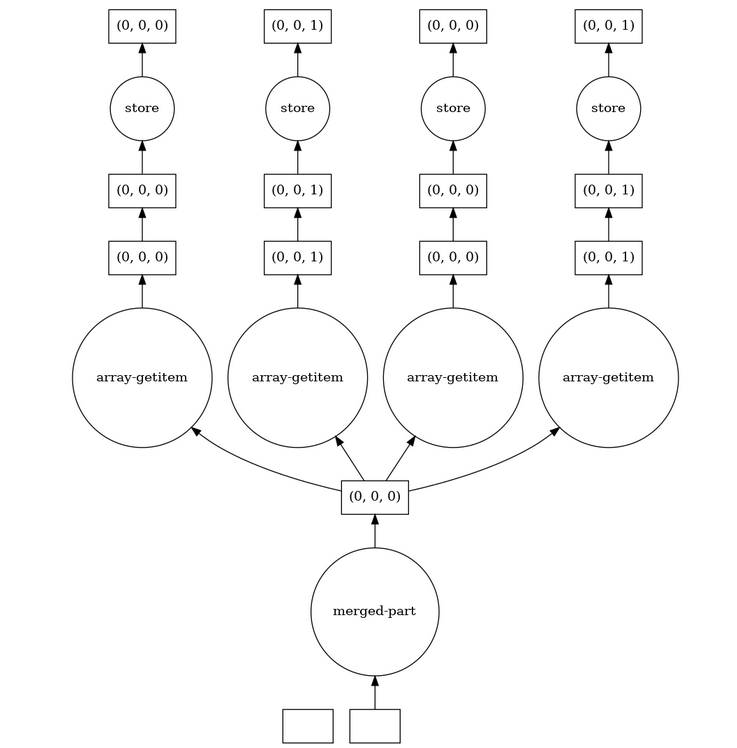
\includegraphics[width=8cm]{./figures/new/after_store.png} }}

  \caption{Optimization of a \texttt{dask} graph of a split using the clustered strategy.}
  \label{fig:bufferization}

\end{figure*}

The optimization starts by converting the task graph into a mathematical
directed graph for use by a BFS (Breadth First Search) algorithm. More
precisely, we implemented it as adjacency lists. The BFS algorithm allows us to
find and store tasks by type for later processing.  Again, the clustered
strategy loads buffers block by block, block columns by block columns or block
slices by block slices~\cite{seqalgorithms}. Assuming that the whole array is
being processed, we find the appropriate buffering scheme from $I$, $O$ and $m$.

We then updated the data loading tasks to force \texttt{dask} to load a whole buffer at
a time instead of small chunks. Finally, we modified the dependent tasks to make
them use our new buffer tasks. According to the clustered algorithm, all buffers
do not necessarily have the same shape, that is why we could not use the
\texttt{dask.array.rechunk} method.

The default scheduler for \texttt{dask.array} is the multi-threaded scheduler. It means
that at the beginning of the execution \texttt{dask} dispatches some tasks that have
no dependencies into different threads. The problem is that the clustered
strategy tries to use all the memory available for each buffer, and such buffer
tasks are the one with no initial dependencies. Therefore, we needed to
modify \texttt{dask}'s scheduler to make it load one buffer only at a time.
This avoids running out of memory during the processing.

\subsection{The keep algorithm}

The buffer extension algorithm described before has been directly
implemented in plain Python. Implementing the last part of the algorithm
consisted in: (1) creating the buffer tasks, (2) dispatching the different data
parts loaded by each buffer into the appropriate output files, (3) simulating
the cache to keep remainders in memory between buffer loadings.

This time, the buffer task creation was straightforward as it is assumed by the
algorithm that the buffers constitute a partition of the whole array. For the
second and third part, we used the \texttt{dask.array.store} method that
requires input arrays as argument, together with the output files in which to
store the data and the indices of each data part in the output files. To
automatically compute such information, we proceeded as follows. We first
compute, for each output file, the list of each constitutive subarrays, with
subarrays defined by the intersection of input and output files and buffers.
When each output file ``knows" which part from which buffer are required, we
merge some of them according to the keep strategy to enforce the fact that
a given data part of a given output file has to be stored at once. By doing this
we create dependencies in the task graph. Such dependency tells \texttt{dask} that it
needs to load two buffers before writing a given subarray for example.

\subsection{Dask repartition}

Both implementations are available in a same Python package called \texttt{dask repartition}. It
contains tests with 99\% coverage and is available on PyPI (The Python Package
Index). \texttt{dask repartition} provides a simple API to use the split, merge and repartition
algorithms described in this study (Figure~\ref{fig:daskrepartition_split}).

\begin{figure}
  \begin{verbatim}
  from dask_io.optimizer as opt
  from opt.cases.case_config import Split

  case = Split(inputfilepath, I)
  case.split_hdf5_multiple(datadir)
  arr = case.get()

  enable_clustering(ONE_GIG * 5)
  arr.compute()
  \end{verbatim}
  \caption{Example code to split a multidimensional array using \texttt{dask repartition}'s clustered strategy implementation'}
  \label{fig:daskrepartition_split}
\end{figure}


%----------------------------------------
\section{Experiments}
%----------------------------------------
This section describes the three experiments we did in this study. All the
results are described in the ``Results" section, and the code of the experiments
is available in a dedicated repository on Github.

\subsection{Baseline experiment}
We first designed
an experiment to prove that \texttt{dask.array} was subject to the seek problem.
To that aim we created a random array from a uniform distribution and stored it
as a HDF5 file for later processing. The array had a shape of
$(1925, 1512, 1750)$ which represents 1/8
of the Big Brain size. The experiment then consisted in splitting and merging
the array with \texttt{dask} using two different chunk shapes: one of them,
$(275,189,250)$, doing more seeks than the other; $(5,1512,1750)$
(Table~\ref{tab:exp1}). We did this experiment on both HDD and SSD to see if the
results were also visible when using an SSD which is suposedly less affected by
seeks. The results of this experiment showed that \texttt{dask} was indeed
subject to the seek problem.

\begin{table}[ht]
 \centering
 \caption{Baseline experiment}

  \begin{tabular}[t]{c c c c}
  \hline
  chunks shape & R partition & nb of chunks & nb voxels/chunk \\
    \hline\hline
    (5,1512,1750) & (385,1,1) & 385 & 13,230,000 \\
    \hline
    (275,189,250) & (7,8,7) & 392 & 12,993,750 \\
    \hline
  \end{tabular}

  \label{tab:exp1}
\end{table}

\subsection{Evaluation of the clustered strategy with dask}
In order to see if we could reduce the split/merge processing time of dask, we
implemented and tested the ``clustered" strategy for splitting and merging
multidimensional arrays. We chose this strategy first because it seemed simpler
to implement. We also know from~\cite{seqalgorithms} that the difference between
the naive and clustered strategies should be large enough to be visible in the
processing time. The shapes used for the experiment are shown on the
Table~\ref{tab:exp2}.

\begin{table}[ht]
 \centering
 \caption{Experiment 2}

  \begin{tabular}[t]{c c c c}
  \hline
    R & chunks shape & buffer size \\
    \hline\hline
    (3500, 3500, 3500) & (875, 875, 875) & 15 GB  \\
    \hline
    (3500, 3500, 3500) & (500, 500, 500) & 15 GB  \\
    \hline
    (3500, 3500, 3500) & (350, 350, 350) & 15 GB  \\
    \hline
    (3500, 3500, 3500) & (50, 3500, 3500) & 15 GB \\
    \hline
    (3500, 3500, 3500) & (28, 3500, 3500) & 15 GB \\
    \hline
  \end{tabular}

  \label{tab:exp2}
\end{table}

\subsection{Evaluation of the keep algorithm}
After these two preliminary experiment, and in order to evaluate the
efficiency of the keep algorithm, we compared it against vanilla \texttt{dask}
on local computer. To be fair we used dask with one thread as required for our
implementation but also with the standard multi-threaded scheduler as it is the
default when using \texttt{dask.array}. In order to compare our implementation
and dask vanilla to a naive repartition, we also added a plain Python implementation
to the benchmark. For the experiments presented below we built a random 3D array
 of the size of Big Brain, drawn from a uniform distribution. Once again, the
 array is initially stored into an HDF5 file.

We did three sub-experiments on the keep algorithm on a multidimensional array
of shape $(3900,3000,3500)$. The first one consisted in comparing the different
implementations in the case where the keep algorithm is supposed to be the most
effective i.e. when the buffer is equal to the input aggregate $B_x=\Lambda_x$
(Table~\ref{tab:exp3_1}). This experiment aimed at showing if the keep
algorithm worked and seeing how much it can improve the processing speed.
The experiment has been done with $I>O$ and $I<O$ at different resolution:
$I~=\frac{R}{5}$, $I~=\frac{R}{10}$, $I~=\frac{R}{22}$ and $I$ of size the size
recommended by \texttt{dask} i.e. more than 100MB (about 200MB in our case).
Note that in Table~\ref{tab:exp3_1} we only tested $I<O$ when $I=(195,150,175)$
as the resulting $O$ size would be too small (less than 10MB).

\begin{table}[ht]
 \centering
 \caption{Experiment 3.1}

  \begin{tabular}[t]{c c c c}
  \hline
    I & O & $I<O$ & B is partition of R \\
    \hline\hline
    (780,600,700) & (650,500,500) & False & True \\
    \hline
    (780,600,700) & (975,1000,875) & True & False \\
    \hline
    (390,300,350) & (325,250,250) & False & True \\
    \hline
    (390,300,350) & (650,500,700) & True & True \\
    \hline
    (195,150,175) & (300,250,250) & True & True \\
    \hline
    (195,150,175) & (650,375,500) & True & False \\
    \hline
    (650,375,500) & (390,300,350) & False & True \\
    \hline
    (650,375,500) & (975,600,700) & True & False \\
    \hline
  \end{tabular}

  \label{tab:exp3_1}
\end{table}

In the second experiment, we tested the case where $m$ is not big enough to get
$B=\Lambda$. We did this experiment at two different resolutions, with $I>O$
and $I<O$ (see Table~\ref{tab:exp3_2}) and tested two buffers for each case:
$B=(1,0.5\Lambda_j,\Lambda_k)$ and $B=(0.5\Lambda_i,\Lambda_j,\Lambda_k)$.
In each case, $B$, $I$ and $O$ must be a partition of $R$. There is one missing
experiment in Table~\ref{tab:exp3_2} as the resulting buffer $B$ was not a
partition of $R$.

\begin{table*}[ht]
 \centering
 \caption{Experiment 3.2}

  \begin{tabular}[t]{c c c c}
  \hline
    $I$ & $O$ & $\Lambda$ & B \\
    \hline\hline
    (780,600,700) & (650,500,500) ($O<I$) & (780,600,700) & (390,600,700) \\
    \hline
    (390,300,350) & (650,500,700) ($O>I$) & (780,600,700) & (390,600,700) \\
    \hline
    (390,300,350) & (325,250,250) ($O<I$) & (390,300,350) & (195,300,350) \\
    \hline
  \end{tabular}
  \label{tab:exp3_2}
\end{table*}

Finally, the particular case of an important shape mismatch was tested, where
$O>>I$ and $O<<I$. In both cases the input aggegate will be quite big which is
supposed to be a bad case for the keep algorithm as extending the buffer to
$\Lambda$ will be more complicated. We tested several cases described in
Table~\ref{tab:exp3_3}. As one can see, $O>>I$ and $O<<I$ seems to be pretty
equivalent as in both cases the input aggregate shape is the same. But both are
worth experimenting as when $O<<I$ we only read one file, whereas $O>>I$ implies
that the algorithm has to switch between a lot of input files.

\begin{table*}[ht]
 \centering
 \caption{Experiment 3.3}

  \begin{tabular}[t]{c c c c c}
  \hline
    $I$ & $O$ & $\Lambda$ & B & $x_i$/$x_j$\\
    \hline\hline
    (1950,1500,1750) & (195,150,175) & (1950,1500,1750) & (1,375,$\Lambda_k$) & $x_j=$25\%$\Lambda_j$ \\
    \hline
    (1950,1500,1750) & (195,150,175) & (1950,1500,1750) & (1,750,$\Lambda_k$) & $x_j=$50\%$\Lambda_j$ \\
    \hline
    (1950,1500,1750) & (195,150,175) & (1950,1500,1750) & (390,$\Lambda_j$,$\Lambda_k$) & $x_i=$20\%$\Lambda_i$ \\
    \hline
    (1950,1500,1750) & (195,150,175) & (1950,1500,1750) & (975,$\Lambda_j$,$\Lambda_k$) & $x_i=$50\%$\Lambda_i$ \\
    \hline
    (195,150,175) & (1950,1500,1750) & (1950,1500,1750) & (1,375,$\Lambda_k$) & $x_j=$25\%$\Lambda_j$ \\
    \hline
    (195,150,175) & (1950,1500,1750) & (1950,1500,1750) & (1,750,$\Lambda_k$) & $x_j=$50\%$\Lambda_j$ \\
    \hline
    (195,150,175) & (1950,1500,1750) & (1950,1500,1750) & (390,$\Lambda_j$,$\Lambda_k$) & $x_i=$20\%$\Lambda_i$ \\
    \hline
    (195,150,175) & (1950,1500,1750) & (1950,1500,1750) & (975,$\Lambda_j$,$\Lambda_k$) & $x_i=$50\%$\Lambda_i$ \\
    \hline
  \end{tabular}

  \label{tab:exp3_3}
\end{table*}

\subsection{Experimental setting}
All these experiments have been executed under the same conditions, on a private
cluster using \texttt{slurm} as workload manager. Each compute node has 256GB of
RAM, 6 SSDs of size 480 GB and 32 cores. We only used 1 node and 1 SSD at a
time. The Python environment used was a
conda environment, all packages used together with their version are available
in a \texttt{requirements.txt} file. The instructions about how to install the
dependencies in a virtual or
conda environement are provided in the \texttt{README} file of the
\href{https://github.com/big-data-lab-team/dask_io}{project's repository}. The
code for all experiments can be found in a
\href{https://github.com/GTimothee/dask_io_experiments}{dedicated repository}
as well.
%----------------------------------------
\section{Results}
%----------------------------------------

\subsection{Baseline experiment}
\begin{figure*}
  \centering
  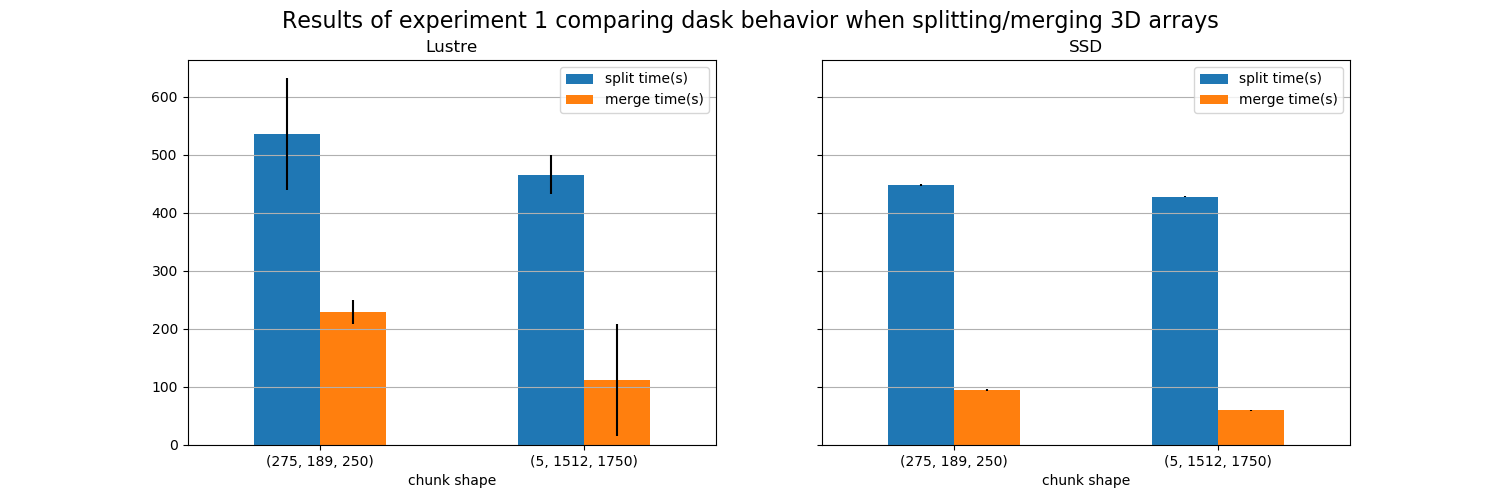
\includegraphics[scale=0.5]{./figures/exp1_results.png}
  \label{fig:exp1}
  \caption{Experiment 1}
\end{figure*}

\subsection{Experiment 2}
\begin{figure*}
  \centering
  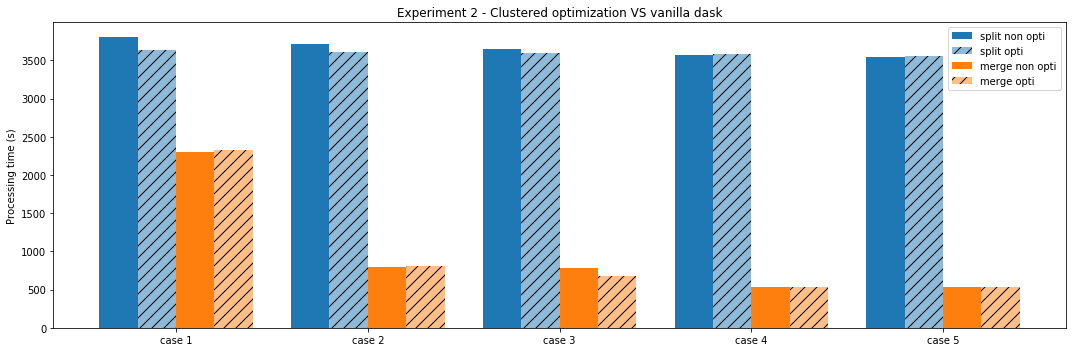
\includegraphics[scale=0.5]{./figures/exp2_results.png}
  \label{fig:exp2}
  \caption{Experiment 3.2  - (chunk shape)\\
  case 1 (350, 350, 350)\\
  case 2 (500, 500, 500)\\
  case 3 (875, 875, 875)\\
  case 4 (28, 3500, 3500)\\
  case 5 (50, 3500, 3500)\\
  }
\end{figure*}

\subsection{Experiment 3}
\subsubsection{Experiment 3.1}
\begin{figure*}
  \centering
  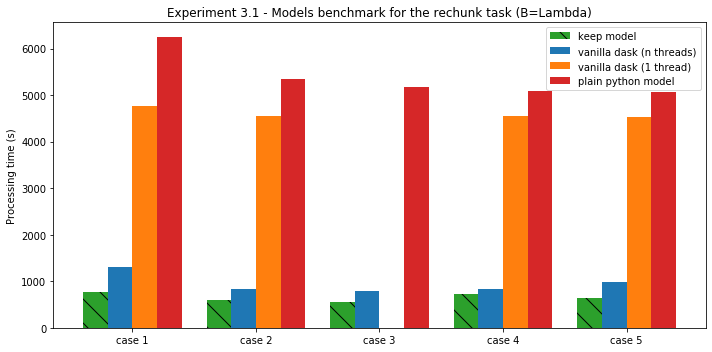
\includegraphics[scale=0.5]{./figures/exp5_1_results.png}
  \label{fig:exp3_1}
  \caption{Experiment 3.1  - (O)(I)(B)\\
  case 1 (300, 250, 250)(195, 150, 175)(390, 300, 350)\\
  case 2 (325, 250, 250)(390, 300, 350)(390, 300, 350)\\
  case 3 (390, 300, 350)(650, 375, 500)(650, 375, 500)\\
  case 4 (650, 500, 500)(780, 600, 700)(780, 600, 700)\\
  case 5 (650, 500, 700)(390, 300, 350)(780, 600, 700)\\
  }
\end{figure*}

Note that the keep algorithm is being run with the single-threaded scheduler.

\subsubsection{Experiment 3.2}
\subsubsection{Experiment 3.3}

%----------------------------------------
\section{Discussion}
%----------------------------------------

\subsection{The buffer ordering problem}
The buffer ordering problem can be modeled as follows: We can represent the
problem as a complete bidirectional graph in which each vertex is a buffer. At
initialization, we must choose a first buffer as an entry point. Let us define
a path in the graph as a visitation order of all buffers in the graph. One buffer
cannot appear twice in the list. Finally, let us define a cache that contains
the data currently in main memory. We define the buffer ordering problem as the
problem of finding the optimal path such that the amount of memory used by the
cache is kept minimal during the process. For each buffer, we load some data
into the cache (reading the buffer) and free some of it (writing into output files). The amount of
data released is different depending of the buffers previously visited and each
buffer can only be visited once which can be represented by removing all edges
pointing to a visited vertex except the one coming from the previously visited
vertex. One may solve this problem by using a greedy algorithm or a shortest path
algorithm but it would
incur more infering at runtime and a potentially complex algorithm to run.
We decided to keep things simple using a naive buffer order, the storage order,
as the goal of this study was primarily to assess if the keep algorithm works.

\subsection{Breaking the buffers}
To even reduce the maximum amount of memory used during the repartition process, we
could read the input files one by one instead of enforcing \texttt{dask} to read a whole
buffer at a time, provided that the input files' parts are read in the right
order (following the buffer order). The idea of reading an entire buffer at a
time came from the clustered and multiple strategies but we realized afterwards
that this could be beneficial to break the buffers into input files' parts. We
can see in Equation (2) that it would result in replacing $B_iB_jB_k$ by
$I_iI_jI_k$ or less if part of a file is loaded. This idea would only be
beneficial in the case where $B_x>I_x$. Indeed, in the other case, the buffer is
loaded anyways.

\subsection{ROI extraction problem}
The Region Of Interest (ROI) extraction problem is a related problem that still needs
to be adressed. A solution using chunking as been introduced in~\cite{optimal_chuking}. The authors
define an array partitioned into chunks of equal shapes and then define a
query as an arbitrary subarray of the input, chunked, array. They define the
optimal chunking problem as finding the optimal chunk such that the expected
number of chunks retrieved to answer the query is minimal. In our opinion, the
solution in~\cite{optimal_chuking} is limited due to the need of historical or theoretical workload
and the necessity to repartition the input array into an ``optimal" chunk shape. We
would prefer letting the application choose the appropriate chunk shape
regarding its needs and not needing to estimate the processing workload. We
define the ROI extraction problem as follows: Finding an algorithm that takes
as input an arbitrary chunk shape and extract the ROI data from the chunks with
the less number of seeks as possible.

\subsection{Solving three problems at once}
As stated in the introduction, the split and merge tasks are special cases of
the repartition task. This observation leads us to think that maybe one could find
one optimal algorithm for the split, merge and repartition tasks.

If we were to use the keep algorithm with $I=R$, we would read the input data
in slices, exactly like the multiple strategy. The only difference between the
two strategies, however, is that if some remainders appear at the bottom of the
buffer, the keep algorithm would keep it to try to read and write files in one
seek. Not only the keep algorithm tries to limit seeking into the files but it
also tries to limit switching between the files. It would be interesting to
compare the two algorithms for the split/merge tasks to see if the keep
implementation brings any kind of improvement.

\subsection{Towards distributed systems}
A future work would be to find distributed versions of the split/merge/repartition
algorithms. Lots of scientists use HPC (High Performance Computing) clusters
regularly which brings considerations about how to use such distributed
algorithms with Lustre for example, a commonly used filesystem for HPC. \texttt{dask}
also provides a distributed scheduler that seems to be quite efficient. It is
now recommended for use, even on local computers (using one node).

%----------------------------------------
\section{Conclusion}
%----------------------------------------

%----------------------------------------
\section{Acknowledgments}
%----------------------------------------

\bibliography{Bibliography}
\bibliographystyle{ieeetr}

\appendices

\section{Memory analysis for the buffer extension algorithm}
\label{bufferExtensionAlgorithm}

Using the nomenclature in section ``The buffer extension algorithm"
(see Figure~\ref{fig:nomenclature_overlaps}), the $x^{th}$ buffer, the volumes'
sizes are:

$\begin{cases}
F_1 = \Omega_k min(B_j, \Theta_j) min(B_i, \Theta_i) \\
F_2 = \Theta_k max(0, min(B_j - \Theta_j, \Omega_j)) min(B_i, \Theta_i) \\
F_3 = \Omega_k max(0, min(B_j - \Theta_j, \Omega_j)) min(B_i, \Theta_i) \\
F_4 = \Theta_k \Theta_j max(0, min(B_i-\Theta_i, \Omega_i)) \\
F_5 = \Omega_k \Theta_j max(0, min(B_i-\Theta_i, \Omega_i)) \\
F_6 = \Theta_k \Omega_j max(0, min(B_i-\Theta_i, \Omega_i)) \\
F_7 = \Omega_k \Omega_j max(0, min(B_i-\Theta_i, \Omega_i))
\end{cases}$

We are only interested in the maximum amount of memory that will be reached by
the algorithm. To that aim, we will not evaluate the above formula for each $x$
but we will replace each $\Omega_d(x)$ by its maximum in $\Sigma$.

In the following paragraphs, we are finding formulas to extend the buffer one
dimension at a time, for use in the buffer stretching algorithm.

\subsection{Formulas of the buffer extension}
\subsubsection{Keeping F1}

We first extend the buffer in the $j$ dimension to keep $F_1$.

\noindent $$F_1 = \Omega_k B_j B_i = \Omega_k B_j$$
$$\Sigma = F_1 + B_iB_jB_k$$
$$\Sigma = B_j (\Omega_k + \Lambda_k)$$
$$\Sigma \leq m \Leftrightarrow B_j (\Omega_k + \Lambda_k) \leq m$$
$$\Sigma \leq m \Leftrightarrow B_j \leq \frac{m}{\Omega_k + \Lambda_k}$$

We define $\phi$, the maximum value for $B_j$:
$$\phi = \lfloor \frac{m}{\Omega_k + \Lambda_k} \rfloor$$

When extending the buffer in the $j$ dimension, $B_i$ stays at 1, so by
definition of $F_1$ the maximum value that $F_1$ can take is $\Omega_k\Theta_j$.
$$B_j = \begin{cases}
  \Theta_j & \textrm{if }\phi \geq \Theta_j \\
  1 & \textrm{if }\phi = 0 \\
  \phi & \textrm{else}
\end{cases}$$

If $B_j=\Theta_j$, then we can continue stretching $B$ in the $j$ direction to
try to keep $F_2$ and $F_3$ areas.

\subsubsection{Keeping F2 and F3}

Let us define $\delta_j$, the amount we will try to add to $B_j$, such that:
$$B_j - \Theta_j = \delta_j$$
$$B_j = \delta_j + \Theta_j$$

From the previous subsection, $F_1$ is of size:
$$F_1 = \Omega_k \Theta_j B_i = \Omega_k \Theta_j$$
$F_2$ and $F_3$ are defined in terms of $\delta_i$:
$$F_2 = \Theta_k \delta_j B_i = \Theta_k \delta_j$$
$$F_3 = \Omega_k \delta_j B_i = \Omega_k \delta_j$$

We get:
$$\Sigma = F_1 + n(F_2+F_3)$$
$$\Sigma = \delta_j\Lambda_k(n+1) + \Theta_j(\Omega_k\Lambda_k)$$
$$\Sigma \leq m \leftrightarrow \frac{m-\Theta_j(\Omega_k\Lambda_k)}{\Lambda_k(n+1)}$$
$$\phi = \lfloor \frac{m-\Theta_j(\Omega_k\Lambda_k)}{\Lambda_k(n+1)} \rfloor$$
$$B_j = \begin{cases}
  \Lambda_j & \textrm{if }\phi \geq \Lambda_j \\
  B_j = \Theta_j & \textrm{if }(B_j+\phi) = 0 \\
  B_j + \phi & \textrm{else}
\end{cases}$$

Again, if $B_j=\Lambda_j$, we continue to stretch the buffer, this time in the
$i$ dimension as $B$ equals $\Lambda$ in the $k$ and $j$ direction.

\subsubsection{Increasing F1, F2 and F3 in the ith dimension}
$$F_1 = \Omega_k\Theta_jB_i$$
$$F_2 = \Theta_k\Omega_jB_i$$
$$F_3 = \Omega_k\Omega_jB_i$$
$$\Sigma = B_i(\Omega_k\Theta_j + n\Omega_j\Lambda_k + \Lambda_j\Lambda_k)$$
$$\Sigma \leq m \leftrightarrow B_i \leq \frac{m}{\Omega_k\Theta_j + n\Omega_j\Lambda_k + \Lambda_j\Lambda_k}$$
$$\phi = \lfloor \frac{m}{\Omega_k\Theta_j + n\Omega_j\Lambda_k + \Lambda_j\Lambda_k} \rfloor$$

$$B_i = \begin{cases}
  \Theta_i & \textrm{if }\phi \geq \Theta_i \\
  1 & \textrm{if }\phi = 0 \\
  \phi & \textrm{else}
\end{cases}$$

If $B_i=\Theta_i$, we continue to stretch the buffer.

\subsubsection{Keeping F4, F5, F6, F7}

$$\begin{cases}
  F_1 = \Omega_k\Theta_j\Theta_i \\
  F_2 = \Theta_k\Omega_j\Theta_i \\
  F_3 = \Omega_k\Omega_j\Theta_i \\
  F_4 = \Theta_k\Theta_j\delta_i \\
  F_5 = \Omega_k\Theta_j\delta_i \\
  F_6 = \Theta_k\Omega_j\delta_i \\
  F_7 = \Omega_k\Omega_j\delta_i \\
  B_i = \Theta_i + \delta_i \\
  B_j = \Lambda_j\\
  B_k = \Lambda_k\\
\end{cases}$$

$$\Sigma = F_1 + n(F_2 + F_3) + N(F_4 + F_5 + F_6 + F_7) + B_iB_jB_k$$
$$\Sigma = F_1 + n(F_2 + F_3) + N(F_4 + F_5 + F_6 + F_7) + (\Theta_i + \delta_i)\Lambda_j\Lambda_k$$
$$\Sigma = \Theta_i(\Omega_k\Theta_j + n\Omega_j\Lambda_k + \Lambda_j\Lambda_k) + (N+1)\delta_i\Lambda_j\Lambda_k$$

$$\Sigma \leq m \leftrightarrow \delta_i \leq \frac{m-\Theta_i(\Omega_k\Theta_j + n\Omega_j\Lambda_k + \Lambda_j\Lambda_k)}{(N+1)\Lambda_j\Lambda_k}$$
$$\phi = \lfloor \frac{m-\Theta_i(\Omega_k\Theta_j + n\Omega_j\Lambda_k + \Lambda_j\Lambda_k)}{(N+1)\Lambda_j\Lambda_k} \rfloor$$

$$B_i = \begin{cases}
  \Lambda_i & \textrm{if }(B_i+\phi) \geq \Lambda_i \\
  B_i = \Theta_i & \textrm{if }\phi = 0 \\
  B_i+\phi & \textrm{else}
\end{cases}$$

The algorithm stops here, as if $B_i=\Lambda_i$, then the buffer has been
successfully stretched to the input aggregate shape, $\Lambda$.

\end{document}
